\documentclass[compress]{beamer}
\usepackage[portuguese]{babel}
\usepackage{listings}
\usepackage{metalogo}
\usepackage{listings}
\usepackage{fontspec}
\usepackage{tikz}

%\usetheme{Nord}
\usetheme[style=dark]{Nord}
\setmainfont{Yanone Kaffeesatz}
\setsansfont{Andika New Basic}
\setmonofont{DejaVu Sans Mono}

\AtBeginSection[]
{
  \begin{frame}[c,noframenumbering,plain]
    \tableofcontents[sectionstyle=show/hide,subsectionstyle=show/show/hide]
  \end{frame}
}

\AtBeginSubsection[]
{
  \begin{frame}[c,noframenumbering,plain]
    \tableofcontents[sectionstyle=show/hide,subsectionstyle=show/shaded/hide]
  \end{frame}
}

\title{Near Aloe}
\subtitle{Curso Profissional de Técnico de Gestão e Programação de Sistemas Informáticos}
\author{Diogo Valério nr 5}
\institute{Escola Secundária António Damásio}
\date{\today}

\begin{document}

\begin{frame}[plain,noframenumbering]
  \maketitle
\end{frame}
\begin{frame}{Presentation Roadmap}
    \tableofcontents[]
\end{frame}


\section{What is a Programming Language?}
\begin{frame}{What is a Programming Language?}
A \textbf{programming language} is a formal language comprising a set of instructions that produce various kinds of output.
\end{frame}

\begin{frame}{Examples of Programming Languages}
These are some examples of programming languages:
\begin{itemize}
    \item \textit{\textbf{C}}
    \item \textit{\textbf{Java}}
    \item \textit{\textbf{Python}}
\end{itemize}
\end{frame}

\begin{frame}[fragile]{Purpose of Programming Languages}
Code:
\begin{lstlisting}[language=python]
    name = 'joão'
    print('hello, world ')
    print(name)
    print(5+5)
\end{lstlisting}
output:
\begin{lstlisting}
    hello, world 
    joão
    10
\end{lstlisting}
\end{frame}

\begin{frame}[fragile]{Purpose of Programming Languages}
Code:
\begin{lstlisting}[language=python]
x = 6
if x < 5:
    print('x is lower than five')
else:
    print('x is lower than or equal to five')
\end{lstlisting}
output:
\begin{lstlisting}
    
\end{lstlisting}
\end{frame}

\begin{frame}[fragile]{Purpose of Programming Languages}
Code:
\begin{lstlisting}[language=python]
x = 6
if x < 5:
    print('x is lower than five')
else:
    print('x is lower or equal to five')
\end{lstlisting}
output:
\begin{lstlisting}
    x is lower or equal to five
\end{lstlisting}
\end{frame}
\section{What is a Markup Language?}
\begin{frame}{What is a Markup Language?}
A \textbf{Markup Language} is a system for annotating a document in a way that is syntactically distinguishable from the text.
\end{frame}

\begin{frame}{Examples of Markup Languages}
These are some examples of Markup Languages:
\begin{itemize}
    \item \textit{\textbf{\LaTeX}}
    \item \textit{\textbf{Markdown}}
    \item \textit{\textbf{HTML}}
\end{itemize}
\end{frame}

\begin{frame}[fragile]{Purpose of Programming Languages}
Code:
\begin{lstlisting}
# Title

## Subtitle

hello this is a sentence. 
This is it's continuation.

This is a paragraph

\end{lstlisting}
output:
\begin{figure}
    \centering
    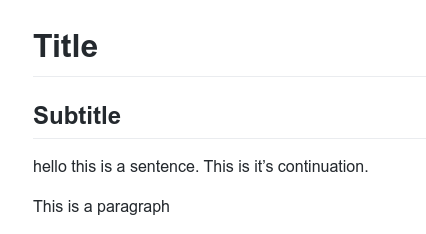
\includegraphics[width=0.5\textwidth]{img/MarkdownPreview.png}
\end{figure}
\end{frame}

\section{why should you use a markup language over other tools?}

\begin{frame}{Simplicity}
    \textbf{Markup} files can be edited by any kind of text/code editor.
\end{frame}
\begin{frame}{Simplicity}
    \begin{figure}
        \centering
        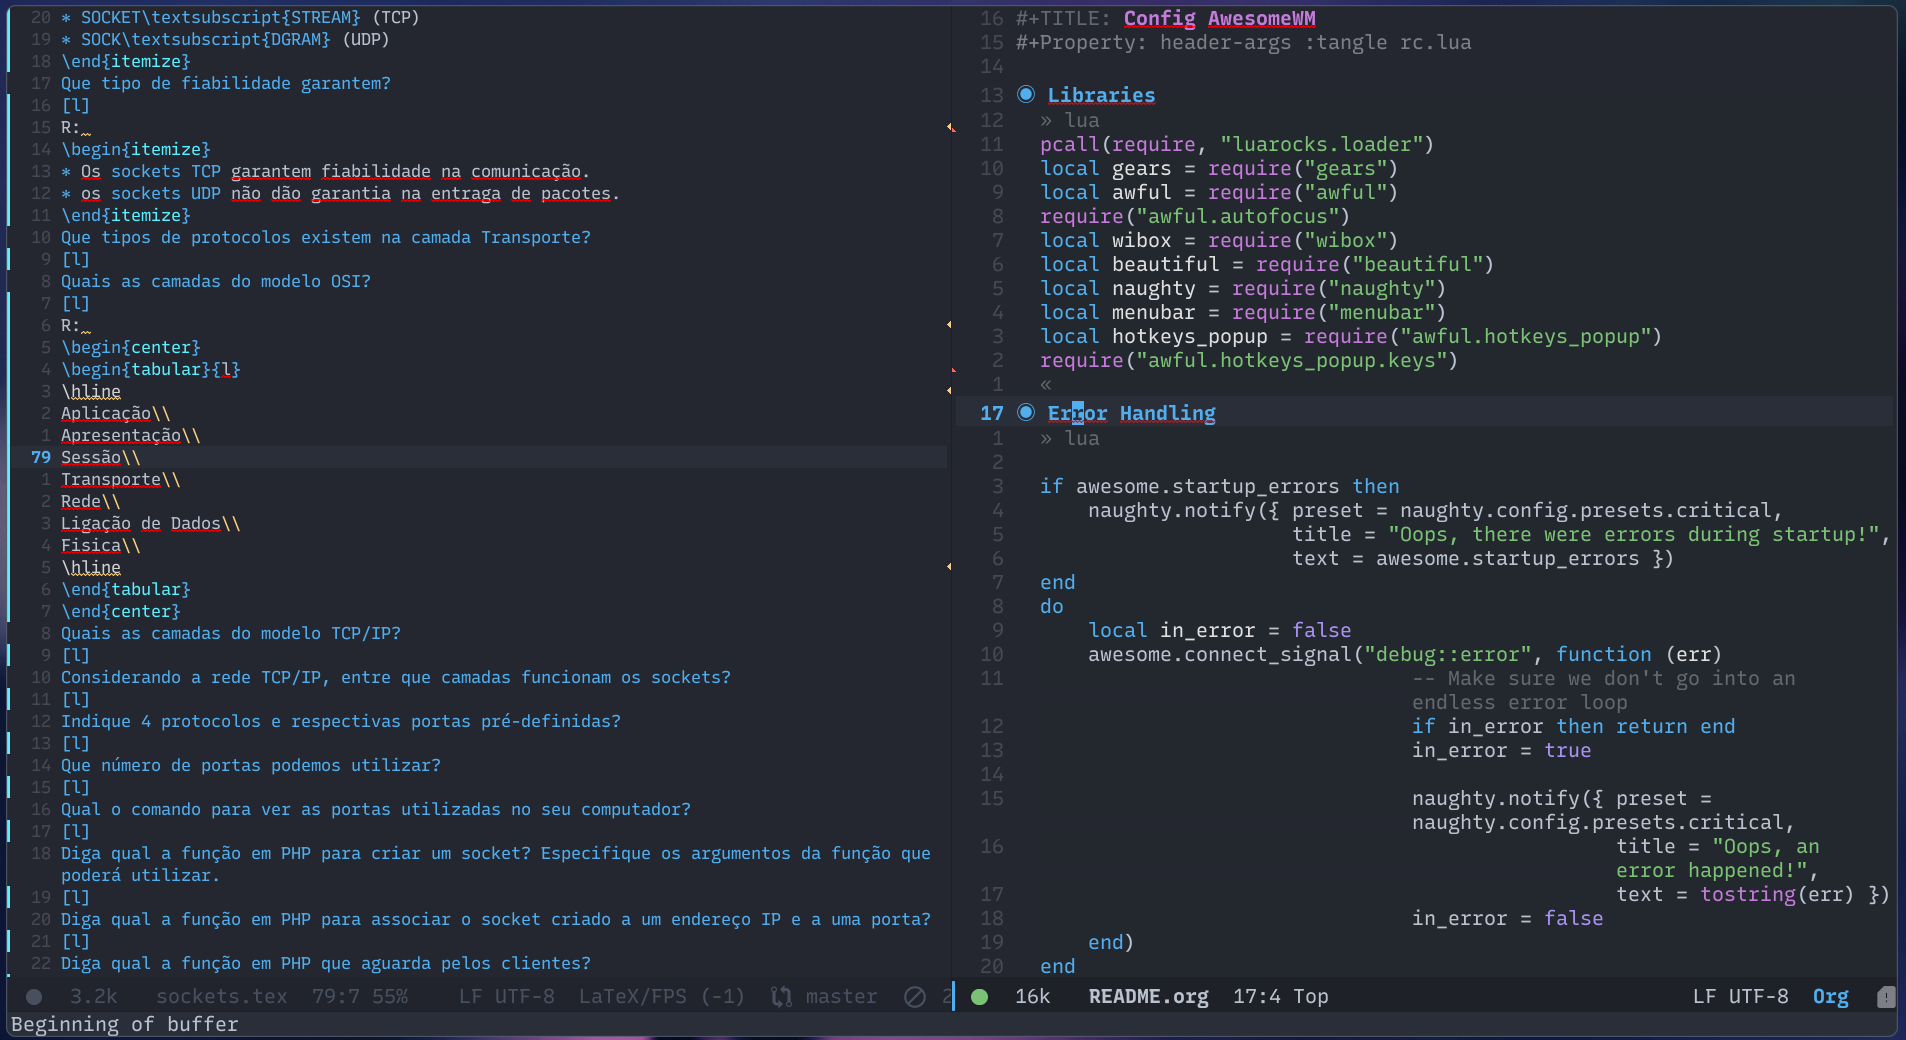
\includegraphics[width=1\textwidth]{img/OQdfAt1.png}
    \end{figure}
\end{frame}
\begin{frame}{Simplicity}
    \begin{figure}
        \centering
        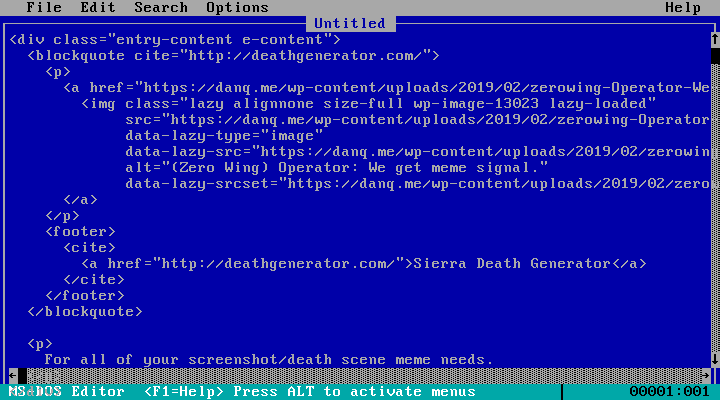
\includegraphics[width=1\textwidth]{img/wpeditcom.png}
    \end{figure}
\end{frame}

\begin{frame}{Low resource usage}
    \textbf{Markup} files can be edited by any kind of  and any kind of machine.
\end{frame}
\begin{frame}{Low resource usage}
    \begin{figure}
        \centering
        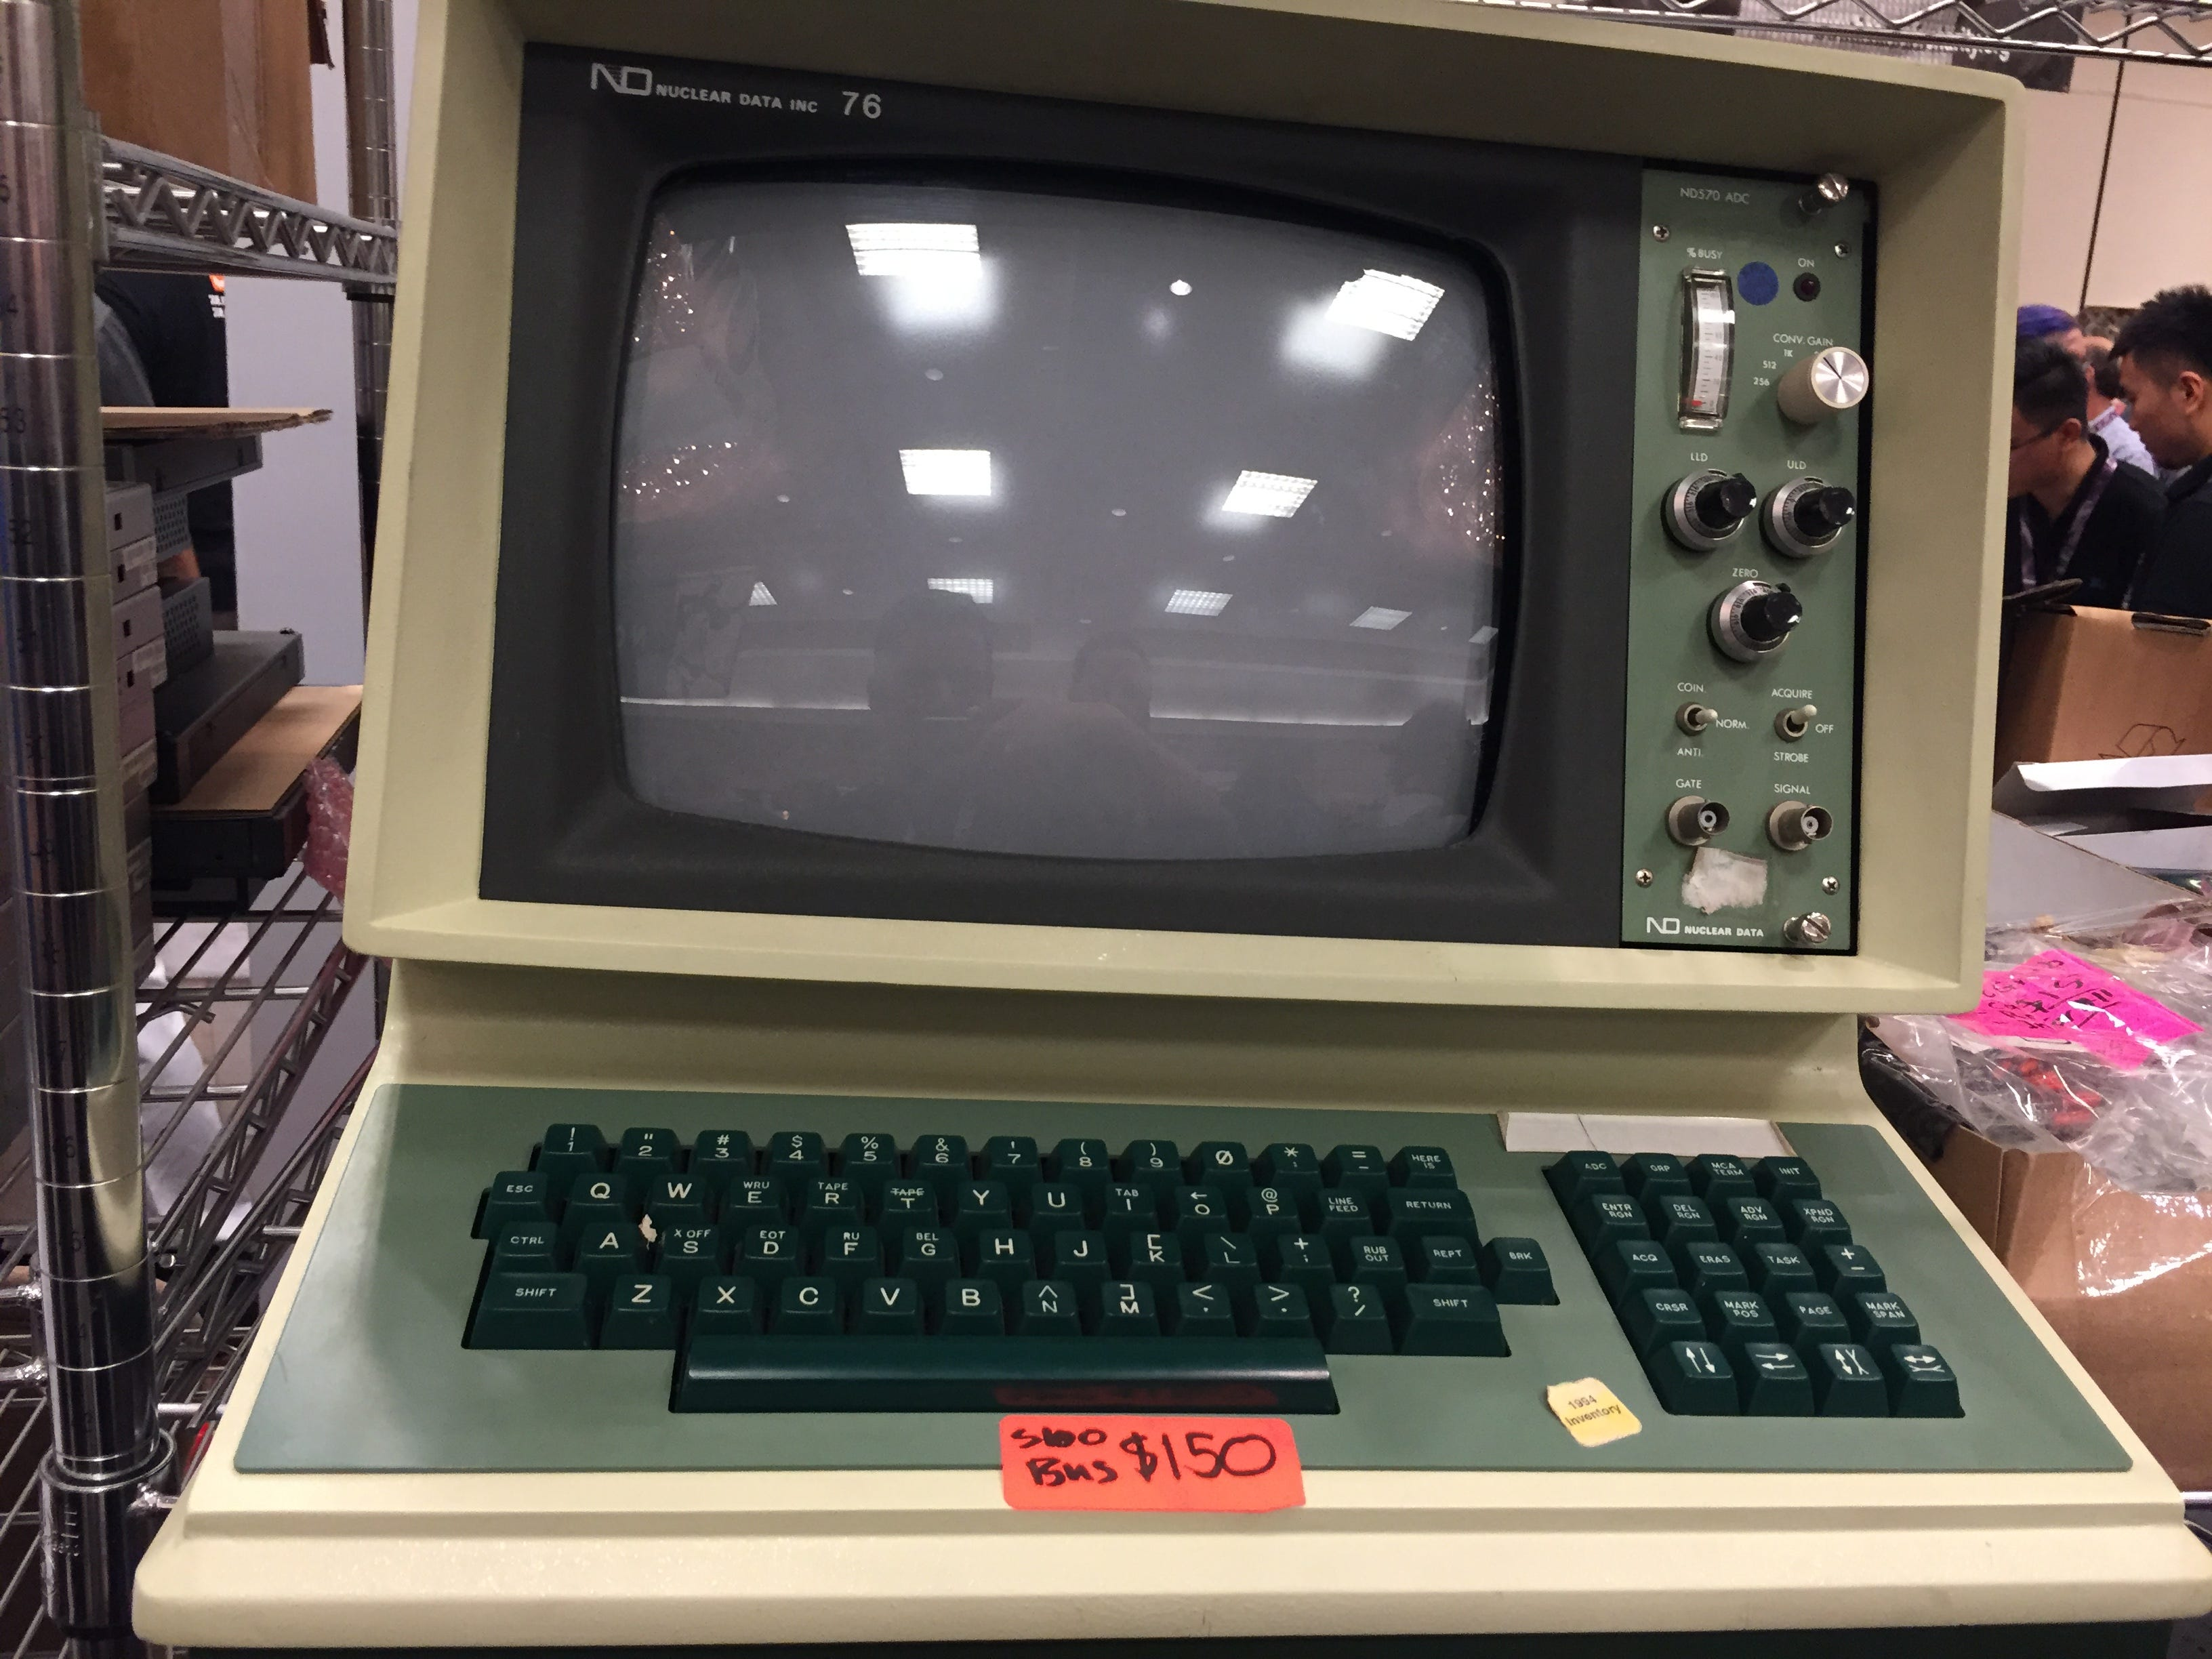
\includegraphics[width=0.6\textwidth]{img/BadPC.jpeg}
    \end{figure}
\end{frame}

\begin{frame}{compatibility}
   Your files will \textbf{never} be a mess again! 
\end{frame}
\begin{frame}{Compatibility}
\begin{figure}
    \centering
    
\includegraphics[width=0.36\textwidth]{img/WindowsMeme.png}
\end{figure}
\end{frame}

\begin{frame}{Ease of use}
    As the size of the files increase the complexity does not evolve exponentially!
\end{frame}
\begin{frame}{Ease of use}
\begin{figure}
    \centering
    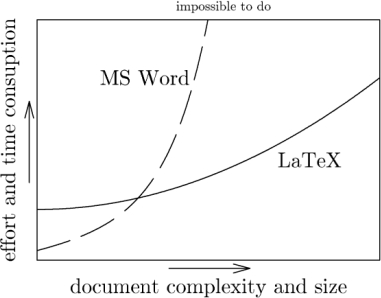
\includegraphics[width=0.7\textwidth]{img/wordvslatex.png}
\end{figure}
\end{frame}

\begin{frame}{}

    \huge{Thanks for your time}
\end{frame}


\end{document}

%%% Local Variables:
%%% mode: latex
%%% TeX-master: t
%%% TeX-engine: xetex
%%% End:
